\chapter{Introduction}

A variable annuity (VA) is a life insurance product created by insurance companies to address concerns that many people have about outliving their assets. Essentially, a VA is a deferred annuity with two phases: the accumulation phase and the payout phase. During the accumulation phase, the policyholder makes purchase payments to the insurance company. During the payout phase, policyholders receive benefit payments from the insurance company. The policyholder has the option of allocating his investments among a set of investment funds. 

A major feature of a variable annuity is that it includes guarantees or riders. These can be divided into two broad categories: death benefits and living benefits. A guaranteed minimum death benefit (GMDB) guarantees a specified lump sum to the beneficiary upon the death of the policyholder regardless of the performance of the investment portfolio. There are several types of living benefits, which include the guaranteed minimum withdrawal benefit (GMWB), the guaranteed minimum income benefit (GMIB), the guaranteed minimum maturity benefit (GMMB), and the guaranteed minimum accumulation benefit (GMAB). A GMWB guarantees that policyholders can make systematic annual withdrawals of a specified amount from the benefit base over a period of time, even though the investment portfolio might be depleted. A GMIB guarantees that policyholders can convert the greater of the current account value or the benefit base to an annuity according to a specified rate. A GMMB guarantees that policyholders received a specific amount at the maturity of the contract. A GMAB guarantees that policyholders can renew the contract during a specified window after a specified waiting period (usually 10 years).

\begin{figure}
  	\begin{subfigure}[b]{0.5\textwidth}
    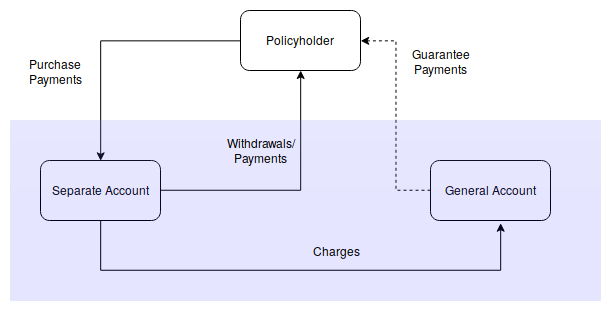
\includegraphics[width=\textwidth]{pictures/novais1.png}
    \caption{Variable annuity flowchart}
    \label{fig:1}
  	\end{subfigure}
  	%
  	\begin{subfigure}[b]{0.5\textwidth}
    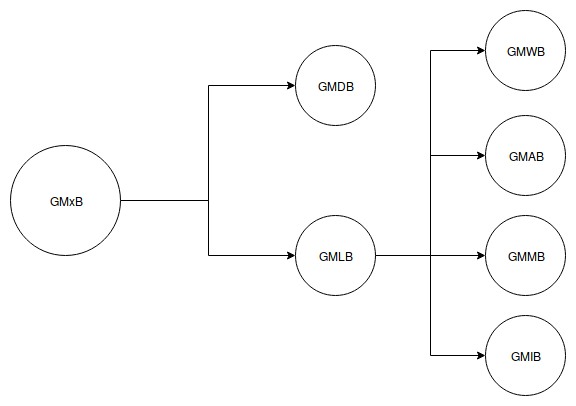
\includegraphics[width=\textwidth]{pictures/novais2.png}
    \caption{Guarantees}
    \label{fig:2}
  	\end{subfigure}
  	\caption{Variable Annuities Description}
\end{figure}


Using dynamic hedging to mitigate the financial risks associated with VA guarantees, insurance companies need to estimate the fair market value (FMV) of guarantees for a large portfolio of VA contracts in a timely manner. 
%Dynamic hedging requires calculating the dollar Deltas of a portfolio of variable annuity policies within a short interval. 
As the value of the guarantees cannot be determined by closed-form formulas, Monte Carlo (MC) simulations are used to value VA portfolios. This approach can be extremely time-consuming as every contract needs to be projected over many scenarios for a long time horizon. To address this computational problem, metamodeling approaches have been proposed.

Metamodeling approaches can significantly reduce the computational effort in the valuation of a large portfolio of VA contracts for two main reasons: first, only a small group of representative contracts needs to be valued using Monte Carlo simulations; second, metamodels are usually simpler and faster than Monte Carlo simulation models. The basic four steps to build a metamodel are illustrated in Figure~\ref{metamodeling}. They consist in: (1) defining a subset of representative VA contracts, (2) computing the FMV for this representative set using MC simulations, (3) fitting a model based on the characteristics and FMV of the contracts, (4) using the estimated model to predict the FMV of the remaining VA contracts. 

\begin{figure}[ht]
\begin{center}
  	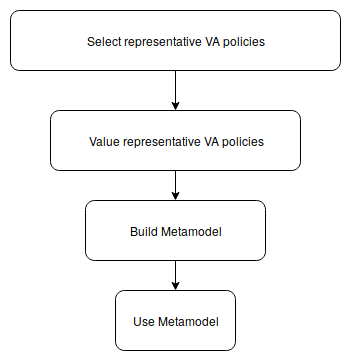
\includegraphics[width=0.4\textwidth]{pictures/novais3.png}
    \caption{Metamodel fluxogram}\label{metamodeling}
\end{center}
\end{figure}



